% Number 400
% UFPM
% Airplane climb Fnet direction
% MIT

% Watermark
\AddToShipoutPicture*{\BackgroundPic}

\addtocounter {ProbNum} {1}

\begin{floatingfigure}[r]{.35\textwidth}
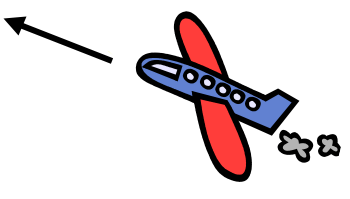
\includegraphics[scale=.5]{/Users/jgates/desktop/latex/pics/airplaneclimb.png}
\end{floatingfigure}
 
{\bf \Large{\arabic{ProbNum}}} An airplane is gaining height as indicated. The airplane is slowing down.

\bigskip
Which of these vectors could be the direction of the net force on a passenger in the plane? Explain!

\setlength{\unitlength}{1mm}
\begin{picture}(100, 40)
  \thicklines
  \put(20, 20){\vector(-2, 1){20}}
  \put(30, 30){\vector(2, -1){20}}
  \put(65, 35){\vector(0, -2){20}}
  \put(95, 35){\vector(-1, -2){10}}
\end{picture}


%\begin{center}
%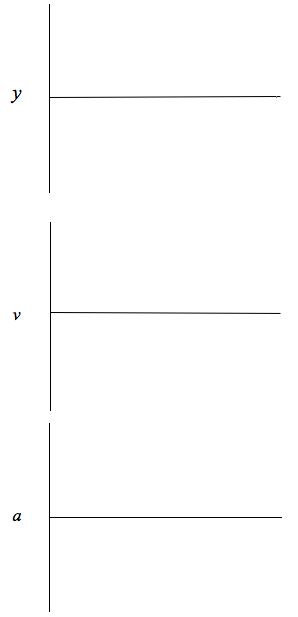
\includegraphics[scale=.85]{/Users/jgates/desktop/latex/pics/blankyvagraphstack.png}
%\end{center}


\vfill
\newpage